\documentclass[compress,mathserif,xcolor=table]{beamer}
\usetheme{sthlm}

%-=-=-=-=-=-=-=-=-=-=-=-=-=-=-=-=-=-=-=-=-=-=-=-=
%        LOADING BEAMER PACKAGES
%-=-=-=-=-=-=-=-=-=-=-=-=-=-=-=-=-=-=-=-=-=-=-=-=

\usepackage{
booktabs,
datetime,
dtk-logos,
graphicx,
multicol,
pgfplots,
ragged2e,
tabularx,
tikz,
wasysym,
multirow,
float,
caption,
subcaption,
amsmath,
mathptmx,
animate
}

\usepackage[scaled=0.9]{helvet}
\usepackage{courier}

\usefonttheme[onlymath]{serif}

\definecolor{mygreen}{RGB}{113, 166, 70}
\definecolor{myblue}{RGB}{68, 140, 185}
\definecolor{myred}{RGB}{217, 98, 55}
\definecolor{mypurple}{RGB}{83, 65, 126}
\definecolor{solviaveis}{RGB}{188, 207, 241}
\definecolor{bronze}{rgb}{0.8, 0.5, 0.2}

\pgfplotsset{compat=1.8}

\usepackage[utf8]{inputenc}
\usepackage[portuguese]{babel}
\usepackage[T1]{fontenc}
\usepackage{newpxtext,newpxmath}
\usepackage{listings}

\lstset{ %
language=[LaTeX]TeX,
basicstyle=\normalsize\ttfamily,
keywordstyle=,
numbers=left,
numberstyle=\tiny\ttfamily,
stepnumber=1,
showspaces=false,
showstringspaces=false,
showtabs=false,
breaklines=true,
frame=tb,
framerule=0.5pt,
tabsize=4,
framexleftmargin=0.5em,
framexrightmargin=0.5em,
xleftmargin=0.5em,
xrightmargin=0.5em
}



%-=-=-=-=-=-=-=-=-=-=-=-=-=-=-=-=-=-=-=-=-=-=-=-=
%        LOADING TIKZ LIBRARIES
%-=-=-=-=-=-=-=-=-=-=-=-=-=-=-=-=-=-=-=-=-=-=-=-=

\usetikzlibrary{
backgrounds,
mindmap
}

%-=-=-=-=-=-=-=-=-=-=-=-=-=-=-=-=-=-=-=-=-=-=-=-=
%        BEAMER OPTIONS
%-=-=-=-=-=-=-=-=-=-=-=-=-=-=-=-=-=-=-=-=-=-=-=-=

\setbeameroption{show notes}

%-=-=-=-=-=-=-=-=-=-=-=-=-=-=-=-=-=-=-=-=-=-=-=-=
%        BEAMER COMMANDS
%-=-=-=-=-=-=-=-=-=-=-=-=-=-=-=-=-=-=-=-=-=-=-=-=


%-=-=-=-=-=-=-=-=-=-=-=-=-=-=-=-=-=-=-=-=-=-=-=-=
%
%	PRESENTATION INFORMATION
%
%-=-=-=-=-=-=-=-=-=-=-=-=-=-=-=-=-=-=-=-=-=-=-=-=

\title{Prefixos, sufixos e \\ formação de palavras \\ em inglês}
\subtitle{DCE747 - Inglês Técnico}
%\date{\small{\jobname}}
\author{\texttt{Iago Carvalho}}
\institute{\texttt{Departamento de Ciência da Computação}}

\hypersetup{
pdfauthor = {Iago A. Carvalho},      
pdfsubject = {Inglês Técnico},
pdfkeywords = {},  
pdfmoddate= {D:\pdfdate},          
pdfcreator = {WriteLaTeX}
}

\begin{document}

\begin{frame}
\titlepage

\end{frame}

%% --------------------------------------------------------

\begin{frame}{Morfologia}

Morfologia é o estudo de formação de palavras em um idioma

\vspace{0.5cm}

Serve para demonstrar a flexibilidade e adaptabilidade do idioma

\vspace{0.5cm}

Regras de formação de palavras são diferentes para cada idioma
\begin{itemize}
    \item Entretanto, normalmente elas se baseiam em 4 coisas
    \begin{enumerate}
        \item Conversão
        \item Composição
        \item Adição de prefixos
        \item Adição de sufixos
    \end{enumerate}
\end{itemize}
\end{frame}

%% --------------------------------------------------------

\begin{frame}{Conversão}

É a estrutura mais simples de formação de palavras em Inglês

\vspace{0.5cm}

A conversão muda o sentido da palavra sem que seja necessária nenhuma alteração

\vspace{0.5cm}

Exemplo: A palavra \textit{drive}
\begin{itemize}
    \item \textbf{Verbo}: He is driving a car
    \item \textbf{Substantivo}: They went to a drive across the country
\end{itemize}
\end{frame}

%% --------------------------------------------------------

\begin{frame}{Composição}

Junção de duas ou mais palavras para a formação de uma nova

\vspace{0.5cm}

\textbf{Teapot} (Bule de chá)
\begin{itemize}
    \item Tea (chá) + pot (panela, vaso)
\end{itemize}

\textbf{Armchair} (poltrona)
\begin{itemize}
    \item Arm (braço) + chair (cadeira)
\end{itemize}

\textbf{Sunglass} (óculos escuros, óculos de sol)
\begin{itemize}
    \item Sun (sol) + glass (vidro, copo, óculos)
\end{itemize}

\textbf{Highway} (rodovia)
\begin{itemize}
    \item High (alto) + way (caminho, maneira, passagem)
\end{itemize}

\end{frame}

%% --------------------------------------------------------

\begin{frame}{Prefixos e sufixos}

Estes são pequenas estruturas adicionadas a outras palavras
\begin{itemize}
    \item É um tipo especial de composição
    \item Prefixos e sufixos tem um significado
    \begin{itemize}
        \item Podem ser adicionados a diversas palavras diferentes
    \end{itemize}
\end{itemize}

\vspace{0.75cm}

\centering 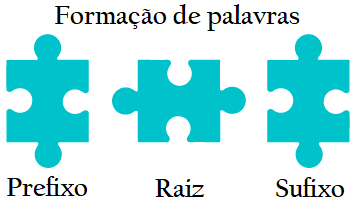
\includegraphics[width=0.75\textwidth]{images/formacao_palavras.png}
\end{frame}

%% --------------------------------------------------------

\begin{frame}{Prefixos}

Prefixos tem papel semântico
\begin{itemize}
    \item Sua adição altera o significado da palavra base
\end{itemize}

\vspace{0.5cm}

A adição de prefixos não altera a grafia da palavra base

\vspace{0.5cm}

Entretanto, em alguns casos, utiliza-se um hifen
\begin{itemize}
    \item Girlfriend $\rightarrow$ ex-girlfriend
    \item Designed $\rightarrow$ well-designed
    \item Conscious $\rightarrow$ self-conscious
\end{itemize}
\end{frame}

%% --------------------------------------------------------

\begin{frame}{Principais prefixos}

\begin{enumerate}
    \item \textbf{ANTI-}: Ideia de combater, de contra
    \begin{itemize}
        \item Virus / Antivirus
        \item Biotic / Antibiotic
        \item Vaxxer (?) / Antivaxxer
    \end{itemize}
    \vspace{1cm}
    \item \textbf{DIS-}: Demonstra oposição a algo
    \begin{itemize}
        \item Like / Dislike
        \item Able / Disable
    \end{itemize}
    \vspace{1cm}
    \item \textbf{IN-, IM-, IR-}: Expressam negação
    \begin{itemize}
        \item Possible / Impossible
        \item Correct / Incorrect
        \item Regular / Irregular
        \item Evitable / Inevitable
    \end{itemize}
\end{enumerate}
\end{frame}

%% --------------------------------------------------------

\begin{frame}{Principais prefixos}

\begin{enumerate}
    \setcounter{enumi}{3}
    \item \textbf{RE-}: Da a ideia de refazer algo, de fazer novamente
    \begin{itemize}
        \item Paint / Repaint
        \item Study / Restudy
        \item Do / Redo
    \end{itemize}
    \vspace{1cm}
    \item \textbf{UN-}: Expressa o não
    \begin{itemize}
        \item Acceptable / Unacceptable
        \item Happy / Unhappy
        \item Avoidable / Unavoidable
        \item Available / Unavailable
    \end{itemize}
    \vspace{1cm}
    \item \textbf{BI-}: Ideia de duplicidade
    \begin{itemize}
        \item Cycle / Bicycle
        \item Lateral / Bilateral
        \item Convex / Biconvex
        \item Sexual / Bisexual
    \end{itemize}
\end{enumerate}
\end{frame}

%% --------------------------------------------------------

\begin{frame}{Sufixos}

Sufixos tem um maior poder do que prefixos
\begin{itemize}
    \item Podem alterar a classe gramatical da palavra
\end{itemize}

\vspace{1.25cm}

Pode ser que um sufixo altere a grafia da palavra base
\begin{itemize}
    \item Happy + -er $\rightarrow$ Happier
\end{itemize}
\end{frame}

%% --------------------------------------------------------

\begin{frame}{Principais sufixos}

\begin{enumerate}
    \item \textbf{-ER}: Comparativo; Da a ideia de "mais \_\_\_ que"
    \begin{itemize}
        \item Tall / Taller
        \item Big / Bigger
        \item Hot / Hotter
        \item Strong / Stronger
    \end{itemize}
    \vspace{0.75cm}
    \item \textbf{-EST}: Forma superlativa; Indica que algo é mais que \textit{TODOS} os outros
    \begin{itemize}
        \item Tall / Tallest
        \item Big / Biggest
        \item Hot / Hottest
        \item Strong / Strongest
    \end{itemize}
    \vspace{0.75cm}
    \item \textbf{-ING}: Modifica o tempo verbal para o gerúndio
    \begin{itemize}
        \item Run / Running
        \item Show / Showing
        \item Act / Acting
    \end{itemize}
\end{enumerate}
\end{frame}

%% --------------------------------------------------------

\begin{frame}{Principais sufixos}

\begin{enumerate}
    \setcounter{enumi}{3}
    \item \textbf{-LY}: Forma adjetivos
    \begin{itemize}
        \item Clear / Clearly
        \item Hour / Hourly
        \item Happy / Happily
    \end{itemize}
    \vspace{0.75cm}
    \item \textbf{-FUL}: Indica que algo é \textit{cheio de}; Que contém muito \_\_\_
    \begin{itemize}
        \item Pain / Painful
        \item Use / Useful
        \item Meaning / Meaningful
    \end{itemize}
    \vspace{0.75cm}
    \item \textbf{-ABLE, -IBLE}: Constrói adjetivos a partir de verbos
    \begin{itemize}
        \item Accept / Acceptable
        \item Afford / Affordable
        \item Comfort / Comfortable
    \end{itemize}
\end{enumerate}
\end{frame}

%% --------------------------------------------------------

\begin{frame}{Outros prefixos e sufixos}

Além destes prefixos e sufixos apresentados, existem diversos outros na língua inglesa

\vspace{0.5cm}

Uma rápida busca na Internet retornará uma grande lista

\vspace{0.5cm}

Também existe um compilado de prefixos e sufixos disponíveis no Github
\href{https://github.com/iagoac/dce747/tree/main/material_apoio}{\beamergotobutton{Link}}
\end{frame}

\end{document}
